\chapter{Introductie op computerarchitectuur}
\label{chap:comparch}
\subsection*{Introductie}
Hoe kan het toch dat we met miljoenen mensen tegelijk naar kattenfilmpjes kunnen kijken op YouTube, elke dag weer? Het antwoord is simpel: de computer. Vermoedelijk hadden de pioniers op computergebied dit specifieke voorbeeld niet verwacht, maar het blijkt dat de computer zich laat lenen voor veel uiteenlopende taken. Dit heeft te maken met de wijze waarop computers zijn opgebouwd, waardoor ze met een paar simpele instructies erg complexe opdrachten kunnen uitvoeren. In dit hoofdstuk kijken we naar de basis van deze opbouw en behandelen we de geschiedenis van de computer en een voorbeeld van een simpele processor.

\subsection*{Leerdoelen}
Na het bestuderen van dit hoofdstuk wordt verwacht dat je:
\begin{itemize}
    % \setlength\itemsep{-1pt}
    \item[--] een aantal mijlpalen uit de geschiedenis van de computerwetenschap kent
    \item[--] de verschillende soorten onderdelen van een computer kent en kunt beschrijven
    \item[--] het concept van een RISC en CISC instructieset kent
    % \item[--] de wet van Moore kent
    \item[--] simpele programma's kunt lezen en programmeren in de 6502 assembleertaal
    \newline
\end{itemize}

% \textit{Relevant materiaal}
Bij dit hoofdstuk hoort hoofdstuk 1 ``Introducing Computer Architecture"\ van het tekstboek van \textbf{Ledin} (\href{https://learning.oreilly.com/library/view/modern-computer-architecture/9781803234519/Text/Chapter\_1.xhtml\#:-:text=Introducing\%20Computer\%20Architecture}{link}).

% \section{Basisbeginselen}

\section{Analytical Engine en voorgangers}

\studeeraanwijzing{Bestudeer in Ledin de paragraaf over de analytical engine,  (\href{https://learning.oreilly.com/library/view/modern-computer-architecture/9781803234519/Text/Chapter\_1.xhtml\#:-:text=Charles\%20Babbage\%E2\%80\%99s\%20Analytical\%20Engine}{link})}

De Analytical Engine van Charles Babbage wordt in \textbf{Ledin} vrij tekstueel beschreven. Hieronder vind je een illustratie van de beschreven machine.

\begin{figure}[!ht]
    \centering
    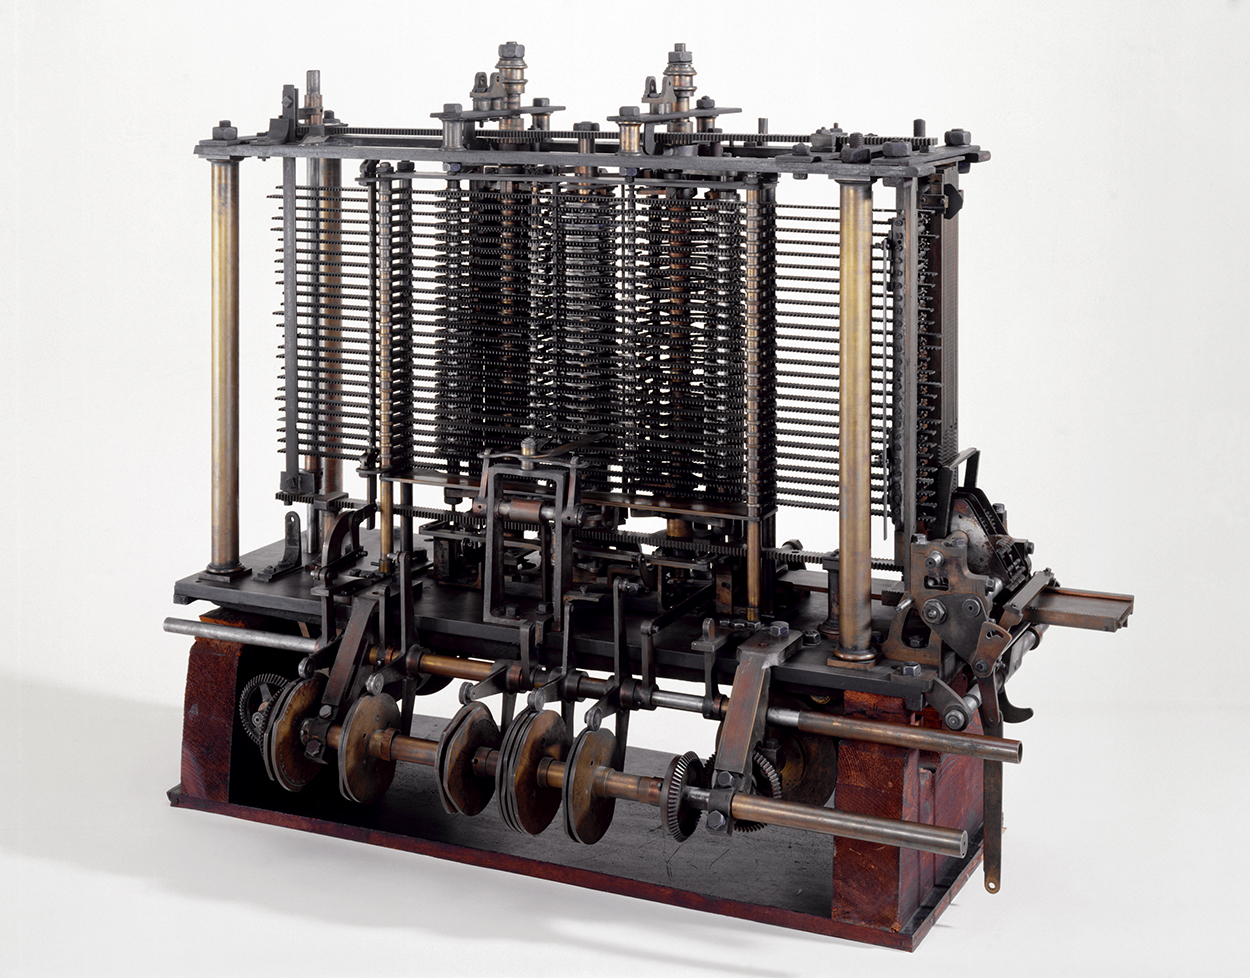
\includegraphics[width=0.6\textwidth]{pictures/figuren/Babbages_Analytical_Engine.jpg}
    \caption{Analytical Engine \\ {\small \textit{Science Museum London, CC BY-SA licentie}}}
    \label{fig:analytical-engine}
\end{figure}

Zoals je kunt zien, verschilt deze machine erg van de computers die we vandaag de dag gewend zijn. Het grootste zichtbare verschil zit hem misschien wel in het feit dat deze machine geen elektrische signalen gebruikt om informatie te representeren, maar dit juist op een mechanische manier probeert op te lossen.

Via de volgende link kun je tevens een leuke YouTube-video bekijken van het kanaal Computerphile, waarin professor David Brailsford een uitleg geeft over deze Analytical Engine: {\color{blue} \url{https://www.youtube.com/watch?v=5rtKoKFGFSM}}.

Zoals professor Brailsford in het filmpje beschrijft, wordt de Analytical Engine geprogrammeerd door middel van een soort ponskaarten. Deze kaarten gebruiken dezelfde techniek als het Jacquardgetouw, een machine welke automatisch bepaalde patronen in stof kan weven aan de hand van dezelfde soort programmeertechniek. Feitelijk is dit weefgetouw geen computer, maar het is wel een voorbeeld van een machine welke te programmeren is om bepaalde handelingen uit te voeren.

Het interessante aan deze technieken is dat ze, hoewel beide al bijna 200 jaar oud, niet de vroegste voorbeelden zijn van computers. Blaise Pascal (1623-1662) heeft in 1642 al een werkende rekenmachine gebouwd. Gottfried Wilhelm von Leibniz (1646-1716) heeft vervolgens dertig jaar na de rekenmachine van Pascal zijn eigen versie gemaakt, welke kon optellen, aftrekken, vermenigvuldigen en delen (de versie van Pascal kon alleen optellen en aftrekken) \cite{tanenbaum}.

Na de Analytical Engine van Babbage zijn er nog een aantal pogingen gedaan om rekenmachines te bouwen. Deze machines gebruikten modernere technieken zoals relais en condensatoren, maar werden op gegeven moment achterhaald door nieuwere technieken zoals het gebruik van vacuümbuizen \cite{tanenbaum}.

\section{Digitale computers}

\studeeraanwijzing{Bestudeer in \textbf{Ledin} de paragraaf over ENIAC (\href{https://learning.oreilly.com/library/view/modern-computer-architecture/9781803234519/Text/Chapter\_1.xhtml\#:-:text=ENIAC}{link}).}

De ENIAC wordt in Ledin beschreven als de eerste programmeerbare digitale computer, maar deze eer gaat eigenlijk naar de COLOSSUS, een computer gebouwd door de Britse overheid tijdens de Tweede Wereldoorlog. Deze computer is gebouwd om berichten te ontcijferen die zijn gecodeerd met een apparaat genaamd SZ40 en SZ42. Zie ook figuur \ref{fig:sz42}.

\begin{figure}[!h]
    \centering
    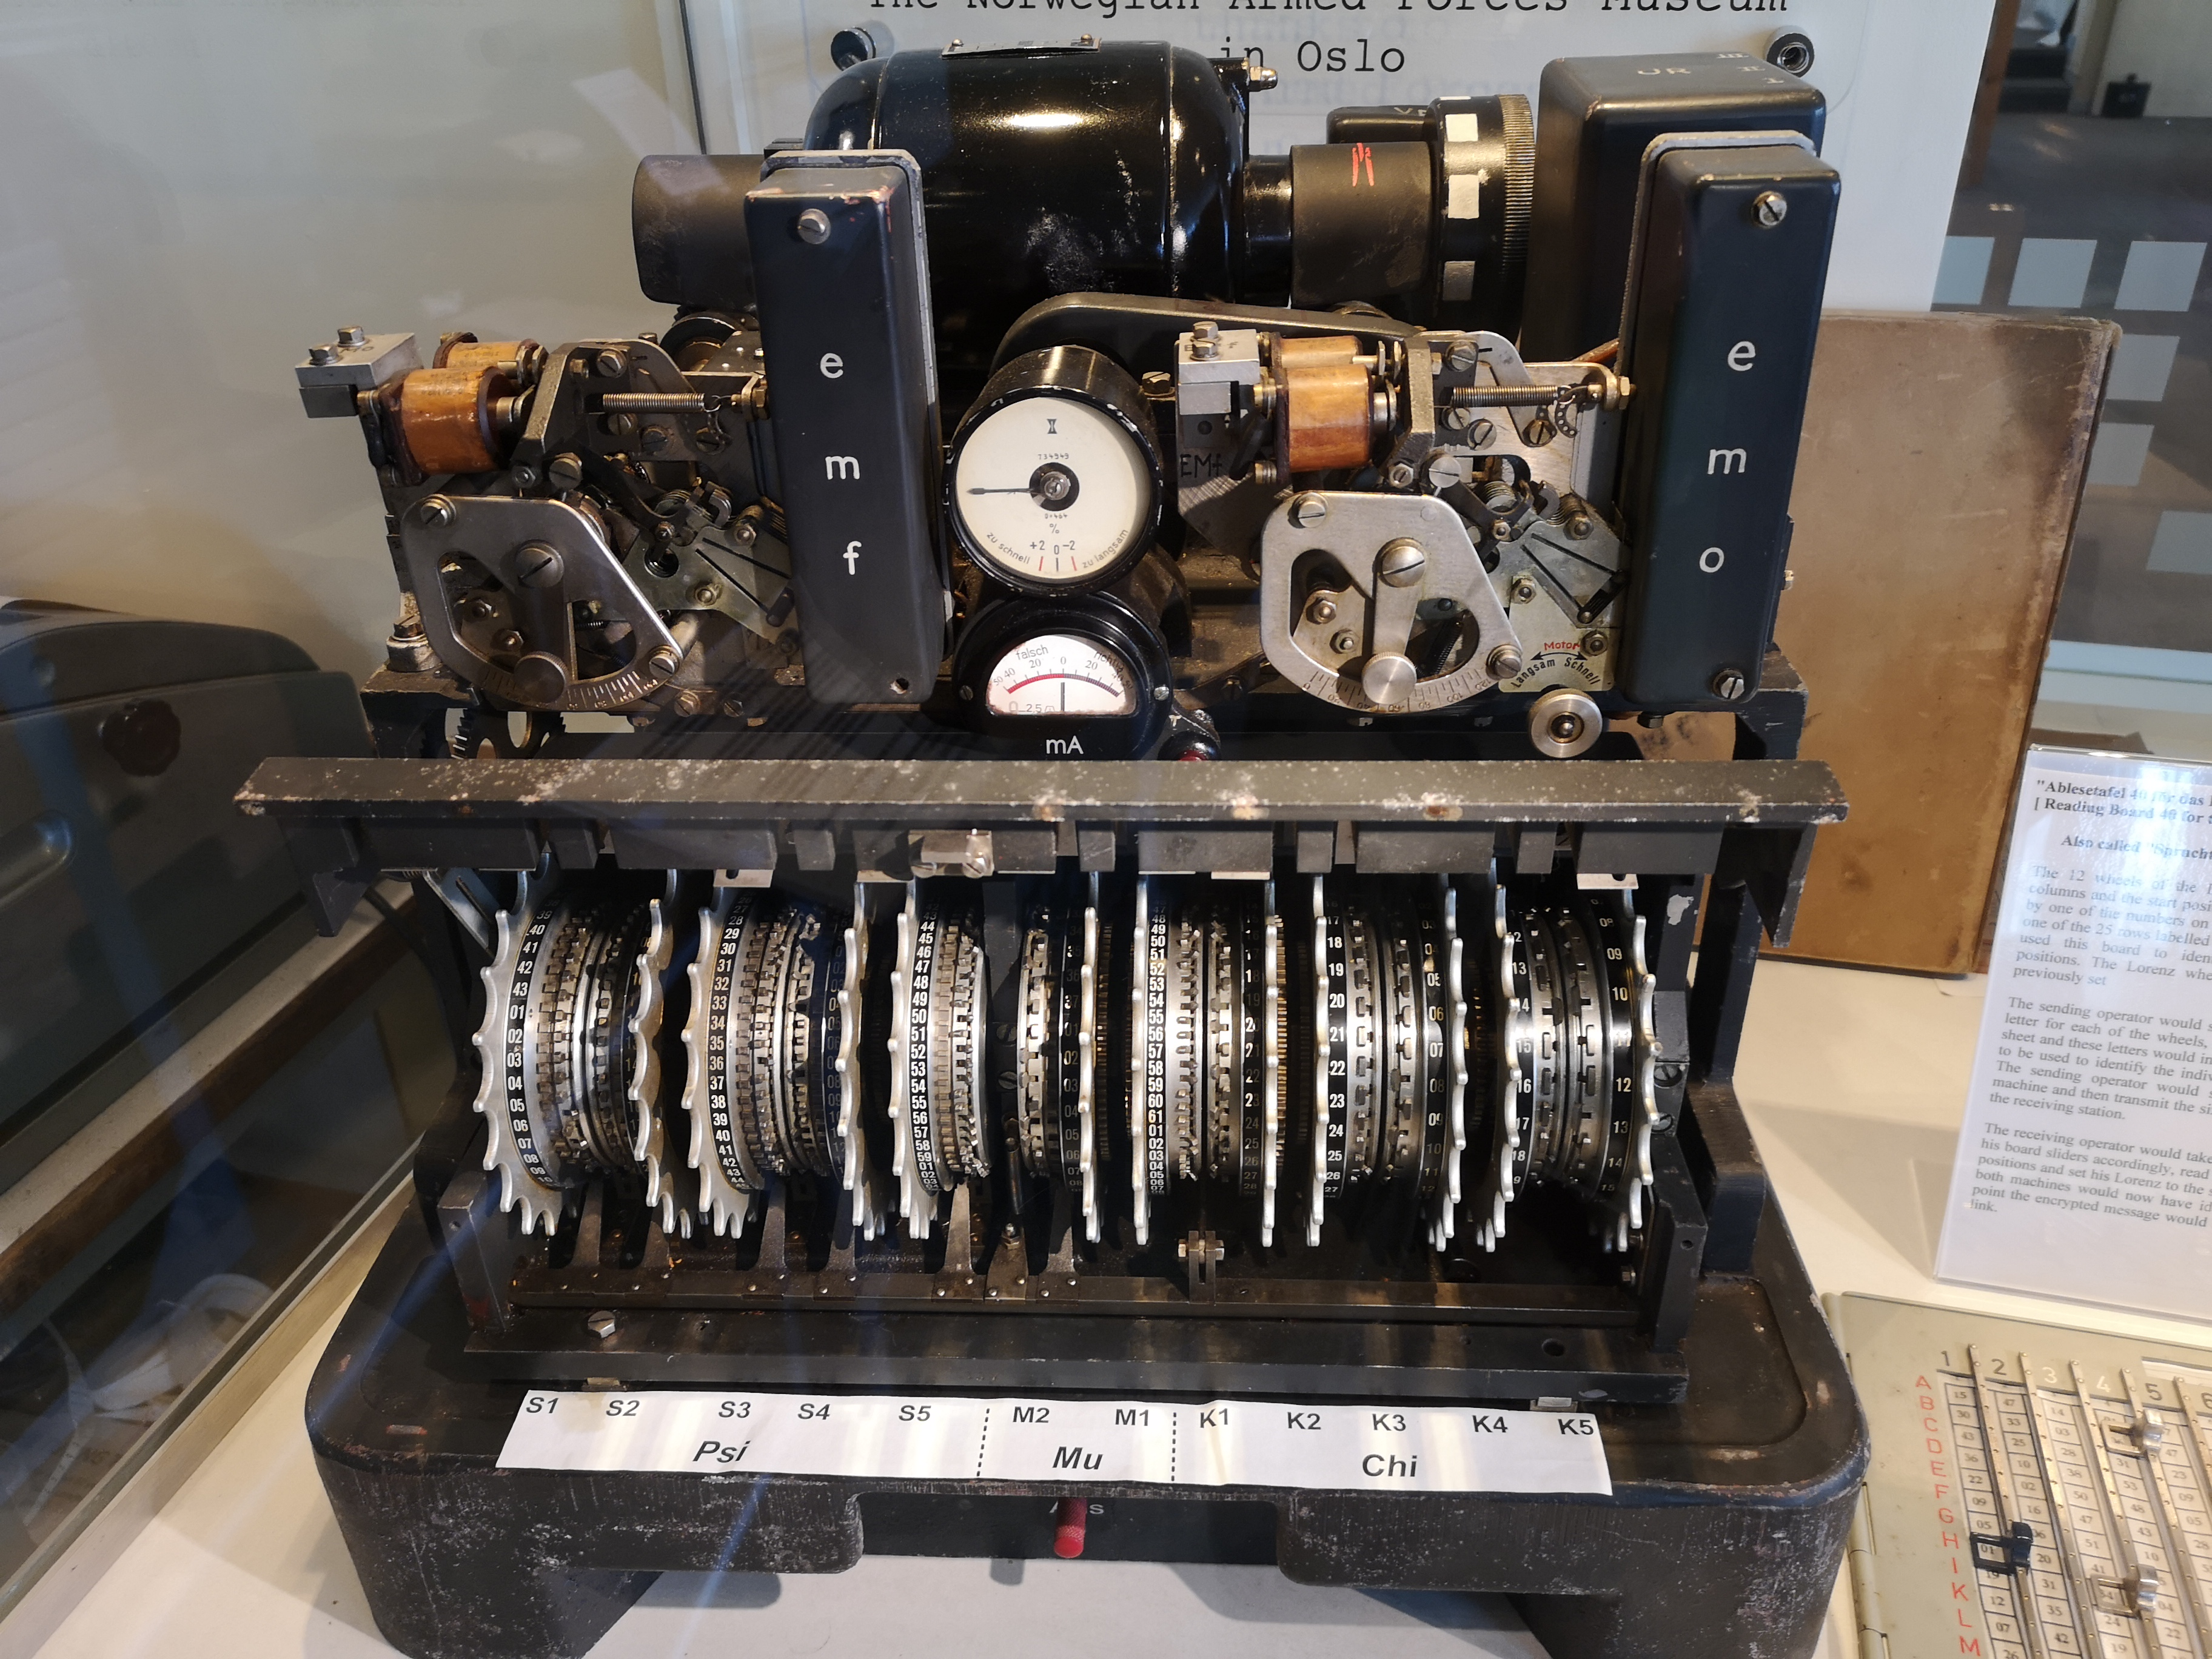
\includegraphics[width=0.5\textwidth]{pictures/figuren/LorenzSZ42at_TNMOC.jpg}
    \caption{SZ42 \\ {\small \textit{TedColes, CC BY-SA licentie}}}
    \label{fig:sz42}
\end{figure}

COLOSSUS is helaas verloren gegaan in de jaren na het einde van de oorlog, omdat de Britse overheid de gebruikte technologie van die tijd geheim wilde houden. De machine is in 1943 in bedrijf gekomen, wat dus iets voor de ENIAC was.

De ENIAC is voor onze standaarden een gigantische computer, zoals ook beschreven in Ledin. Een afbeelding om dit te illustreren vind je in figuur \ref{fig:eniac}. 

\begin{figure}[!h]
    \centering
    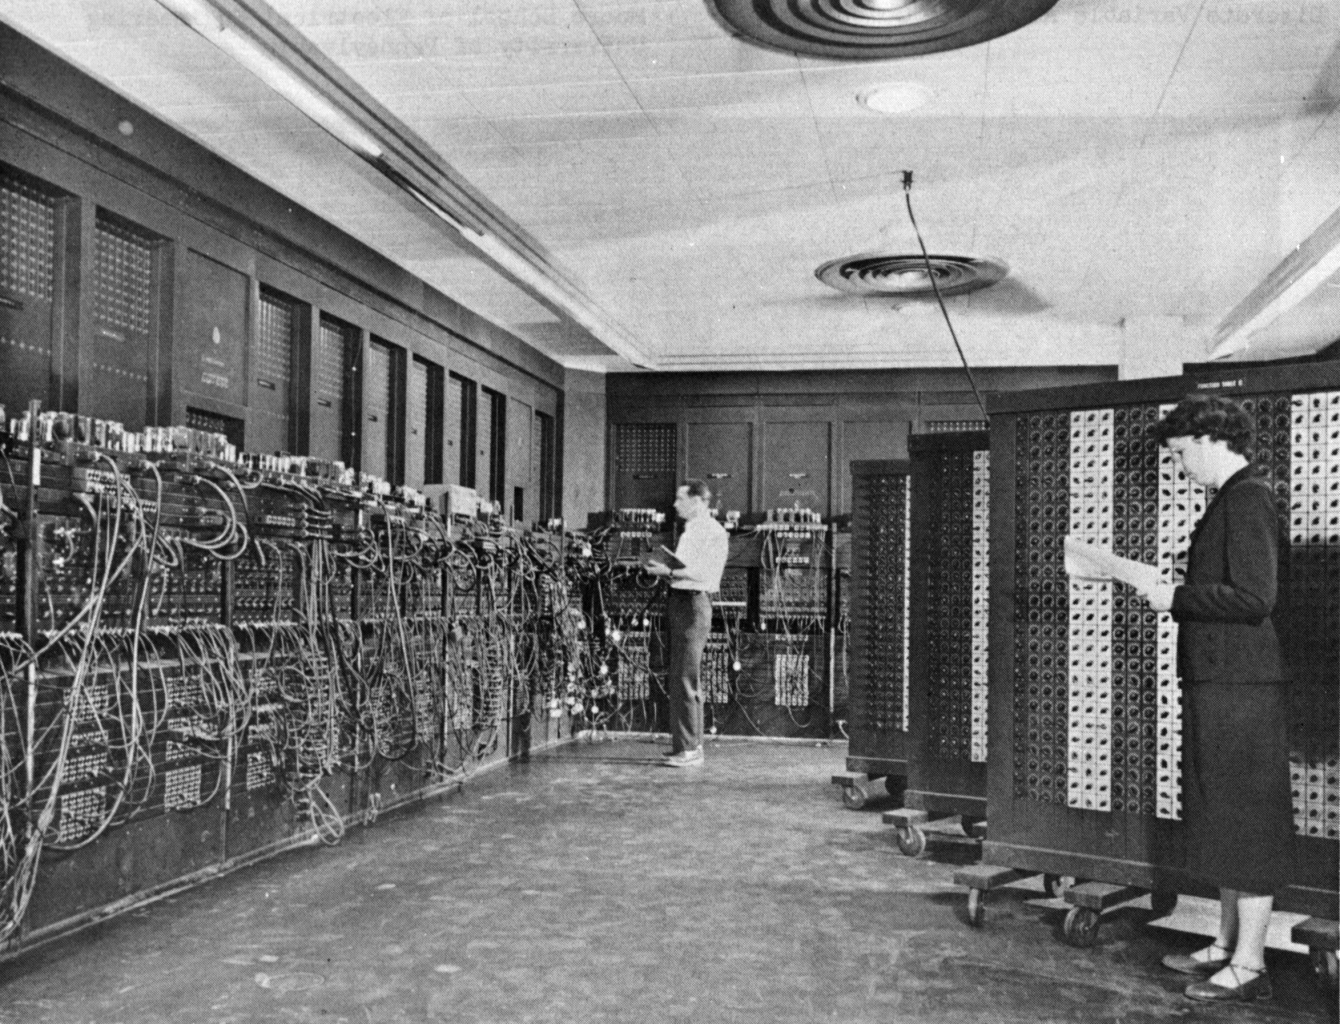
\includegraphics[width=0.75\textwidth]{pictures/figuren/Eniac.jpg}
    \caption{ENIAC \\ {\small \textit{U.S. Army, CC BY-SA licentie}}}
    \label{fig:eniac}
\end{figure}

De ENIAC is gemaakt voor het Amerikaanse leger en was nodig om tijdrovende berekeningen welke eerst met hand werden uitgevoerd, automatisch uit te laten voeren. De machine was pas in 1946 klaar, waardoor het zijn doel mistte omdat de oorlog toen al voorbij was. Toch heeft ENIAC wel een ander, nog veel belangrijker doel behaald: de computer is van grote invloed geweest op andere onderzoekers van die tijd. De makers van de computer hebben een ``zomerschool" mogen houden waarbij ze hun werk toonden aan andere belangstellenden. Dit had een dusdanige invloed dat er in de jaren daarna een aantal op de ENIAC ge\"inspireerde modellen verschenen: EDSAC, JOHNIAC, ILLIAC, MANIAC en WEIZIAC.

John von Neumann heeft tevens meegewerkt als consultant bij de ontwikkeling van de ENIAC. Deze naam zullen we later nog vaker terugzien wanneer we het gaan hebben over de Von Neumann-architectuur.

\subsection{De invloed van de transistor}

\studeeraanwijzing{Bestudeer in \textbf{Ledin} de paragraaf over ``IBM" (\href{https://learning.oreilly.com/library/view/modern-computer-architecture/9781803234519/Text/Chapter\_1.xhtml\#:-:text=In\%20the\%20years\%20following}{link}).}


Het boek van Ledin noemt een aantal technologische mijlpalen binnen de computerarchitectuur. Deze mijlpalen behoren tot het tijdperk waarin de transistor erg belangrijk was. Een aantal machines van uit deze tijd staan hieronder weergegeven, en kunnen uit interesse worden opgezocht.

\begin{table}[!htbp]
\caption{Bekende computers uit 1955-1965}
\label{table:computers55-65}
\small
\begin{tabular}{ l l l l l}
    \cline {1-1} \cline{3-3} \cline{5-5}
    \emph{Computer} & & \emph{Tijdsperiode} & & \emph{Beschrijving}\\
    IBM 7090 &&  1959 && Met transistors uitgevoerde versie van de 709 \\
    PDP-1    && 1961 && Minder snelle computer dan de 7090, maar \\
    && && vele malen goedkoper\\
    PDP-8   && 1965 && Nog goedkoper dan de PDP-1, nu met omnibus\\
    IBM 1401 && 1959 && Kleinere bedrijfscomputer, verkocht erg goed\\
    IBM System/360 && 1965 && Bracht 7090 en 1401 achtige computers in \\
    && && één familie\\
    \cline {1-1} \cline{3-3} \cline{5-5}
\end{tabular}
\end{table}

Het is belangrijk te begrijpen dat de computers in deze tijd nog steeds niet veel leken op de computers die we vandaag de dag gewend zijn. Als voorbeeld kunnen we de IBM 7090 en 1401 nemen. Beide computers werden gemaakt door IBM en je zou verwachten dat beide computers op een soortgelijke wijze geprogrammeerd werden. Men werd op dit punt helaas teleurgesteld omdat de twee computers helemaal niet compatibel waren. Dit zorgt ervoor dat bedrijven soms twee programmeerafdelingen nodig hadden wanneer ze zowel een 7090 als 1401 in dienst hadden.

\subsection{Integrated circuits}

De laatste computer in tabel \ref{table:computers55-65} staat aan het einde van het gegeven tijdperk 1955-1965 en valt ook binnen het daaropvolgende tijdperk: het tijdperk van de integrated circuits (1965-1980). Deze ontwikkeling is belangrijk geweest omdat dit het mogelijk maakte om meerdere transistors op één chip te plaatsen en zo de vorm- en kostenfactor te verkleinen.

\subsection{Personal Computers}

Na de introductie van VLSI (Very Large Scale Integration) werd het mogelijk om heel veel transistors (uiteindelijk miljoenen) op één chip te plaatsen. Tegen de jaren 80 van de vorige eeuw waren de prijzen voor computers zo laag geworden, dat mensen thuis ook een computer konden aanschaffen.

Via de volgende link kun je een interessante YouTube-video bekijken van het kanaal CrashCourse, waarin Carrie Anne een uitgebreide uitleg geeft over de Personal Computer: {\color{blue} \url{https://www.youtube.com/watch?v=M5BZou6C01w}}.

In het filmpje worden de eerste bekende personal computers (Pc's) genoemd. Deze Pc's zijn de computers die het gewone publiek voor het eerst kon kopen naar aanleiding van de prijsdalingen in de branche. De eerste van deze computers waren bedoeld voor hobbyisten en moesten zelf in elkaar worden gezet. Dit was niet voor iedereen weggelegd, waardoor het algemene succes nog uitbleef. Na computers van Apple en Tandy was het aan IBM om de IBM PC te creëren, die zeer populair werd.

\section{Simpele computerarchitectuur}

\studeeraanwijzing{Bestudeer in \textbf{Ledin} het deel over de 8088 en de 80286/80386 (het deel over de iPhone mag je gerust overslaan) (\href{https://learning.oreilly.com/library/view/modern-computer-architecture/9781803234519/Text/Chapter\_1.xhtml\#:-:text=The\%20Intel\%208088\%20microprocessor}{link}).}

Deze stof is lastiger omdat deze technischer van aard is. De volgende uitleg plaatst de stof in context.

\begin{figure}[!h]
    \centering
    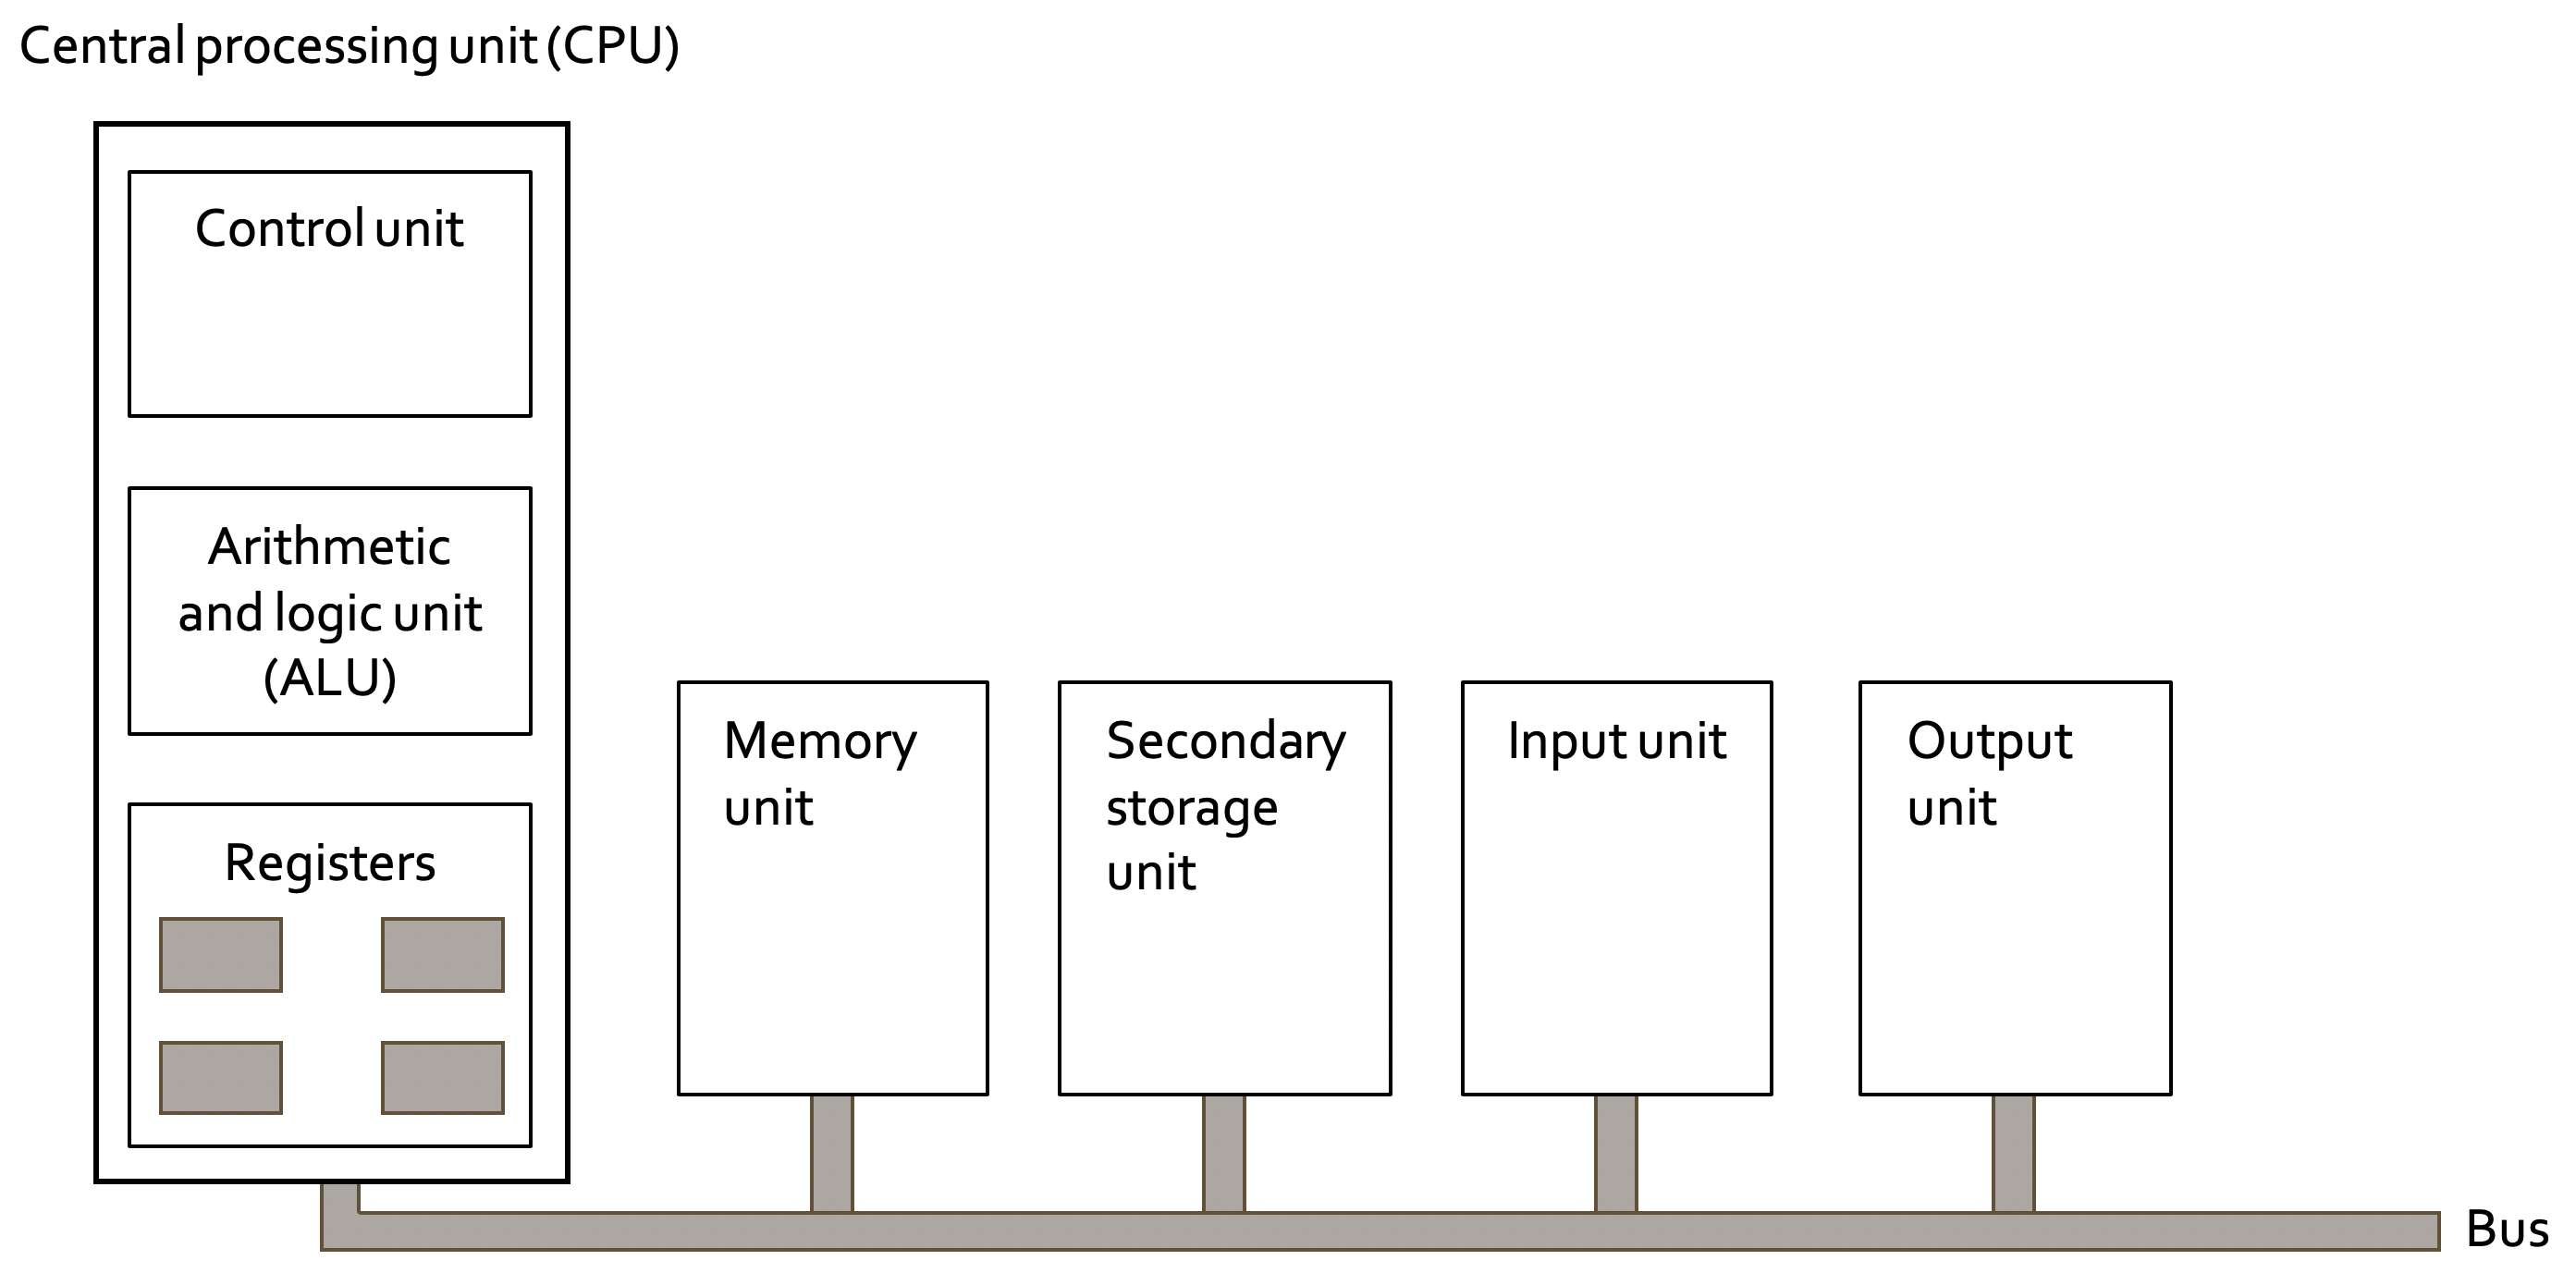
\includegraphics[width=0.95\textwidth]{pictures/figuren/comp_org.png}
    \caption{Versimpelde weergave computerarchitectuur}
    \label{fig:comparch}
\end{figure}

In figuur \ref{fig:comparch} is te zien hoe een simpele computer eruit ziet. Een computer bestaat grofweg uit een aantal onderdelen \cite{tanenbaum}, \cite{deitel-java}:

\begin{itemize}
    \setlength\itemsep{-1pt}
    \item[--] \textbf{Central Processing Unit (CPU)}\\
              De CPU is het hart van de computer. Dit onderdeel voert de opdrachten uit die de computer krijgt in de vorm van de code van een programma. De subonderdelen van de CPU worden hieronder kort behandeld en komen later deels terug.
              \begin{itemize}
                  \item[\textbullet] \textit{Control Unit (Besturingseenheid)}\\
                  De besturingseenheid van de CPU stuurt de computer aan. Deze eenheid houdt zich bezig met het geven van opdrachten aan de andere onderdelen van de computer en het beheren van de Fetch-Decode-Execute Cycle. Dit is de cyclus die de computer constant doormaakt om nieuwe taken uit te voeren binnen het huidige programma. \cite{agarwal}. Deze cyclus begint met het ophalen van het geheugenadres van de instructie die moet worden uitgevoerd, die we de Program Counter noemen (in de intel 8088 heet dit de Instruction Pointer). Deze instructie wordt daarna ingeladen in een speciaal register (het Instruction Register). Eenmaal daar wordt de instructie gedecodeerd (de binnengekomen informatie wordt gelezen en het juiste commando wordt erbij gezocht). Vervolgens wordt de instructie uitgevoerd.
                  \item[\textbullet] \textit{Arithmetic and Logic Unit (ALU)}\\
                  De aritmetische en logische eenheid kan de benodigde berekeningen binnen de computer uitvoeren, zoals optellen, aftrekken, vermenigvuldigen en delen. Ook is apparatuur aanwezig om beslissingen te kunnen nemen, bijvoorbeeld of twee waarden gelijk zijn of niet.
                  \item[\textbullet] \textit{Registers}\\
                  De registers zijn samen een klein en snel geheugen dat gebruikt wordt voor het opslaan van tussenresultaten en bepaalde besturingsinformatie. Elk register heeft zijn eigen functie en zijn allemaal vaak even groot. Daarnaast kan elk register kan één getal bevatten, met een maximale lengte die bepaald wordt door de grootte van het register. Voorbeelden van registers zijn het register voor de Program Counter en het instructieregister.
              \end{itemize}
    \item[--] \textbf{Memory Unit (Primair geheugen)}\\
              Met het hoofdgeheugen van een computer bedoelen we in eerste instantie het geheugen waar de computer mee werkt om snel waarden in op te slaan om deze even later weer te kunnen gebruiken: het RAM (Random Access Memory). Er heeft in de begindagen van de computerwetenschap nog wat onenigheid bestaan over de naamgeving van dit onderdeel. De Britten noemden het een ``store", waar de Amerikanen het ``memory" noemden. Het is duidelijk welke kant we op zijn gegaan. De informatie in dit geheugen bestaat alleen zolang de computer aan staat. Wanneer de computer opnieuw wordt opgestart, is dit geheugen gewist.
    \item[--] \textbf{Secondary Storage Unit (Secundair geheugen)}\\
              Secundair geheugen is de naam die we geven aan geheugen waarin we informatie kunnen opslaan welke wel een herstart van de computer overleeft. Onder deze vorm van geheugen verstaan we bijvoorbeeld een harde schijf of SSD.
    \item[--] \textbf{Input Unit (Invoereenheid)}\\
              De invoereenheid van de computer (ook wel invoereenheden) voorzien de computer van informatie (bijvoorbeeld data en programma). Invoereenheden zijn bijvoorbeeld een keyboard, muis, Dvd-drive, etc.
    \item[--] \textbf{Output Unit (Uitvoereenheid)}\\
              De uitvoereenheid van de computer (ook wel uitvoereenheden) geven de computer de mogelijkheid om informatie beschikbaar te stellen voor gebruik buiten de computer. Uitvoereenheden zijn bijvoorbeeld een computerscherm, printer, etc.
    \item[--] \textbf{Bus}\\
              Een bus is een onderdeel van de computer waarmee adressen, data en stuursignalen kunnen worden verzonden. Bussen kunnen zich binnen de CPU bevinden, maar bevinden zich ook buiten de CPU. De bus uit de afbeelding verbindt de CPU met de verschillende andere onderdelen van de computer, zodat deze met elkaar kunnen communiceren.
\end{itemize}


Via de volgende link kun je een aan te raden YouTubevideo bekijken van het kanaal CrashCourse, waarin Carrie Anne een uitgebreide uitleg geeft over de architectuur van een processor: {\color{blue} \url{https://www.youtube.com/watch?v=rtAlC5J1U40}}.

\subsection{Instructieset}
De toevoeging van de iPhone in Ledin zal niet zonder reden zijn. Het aannemelijkst is dat deze als voorbeeld dient van een apparaat dat een ARM processor gebruikt. ARM (Advanced RISC Machine) is een processor met een kleinere instructieset dan de processors van Intel. Een instructieset is de verzameling van alle commando's die gegeven kunnen worden aan een processor. Hierbij moet gedacht worden aan het niveau van ``haal waarde op van geheugenlocatie \textit{A}", of ``tel waarden in twee registers bij elkaar op". Een processor met een kleiner aantal van deze soort instructies noemen we een RISC-processor (Reduced Instruction Set Computer). 

Een processor met een groot aantal instructies en ook per stuk complexere instructies, noemen een CISC-processor (Complex Instruction Set Computer) \cite{tanenbaum}. Voordelen van een RISC-processor tegenover een CISC-processor zijn van oudsher dat de RISC-processor goedkoper zijn en indertijd ook sneller waren onder bepaalde omstandigheden. Tegenwoordig is dit verschil niet meer zo spannend omdat dezelfde ideeën die hebben geleid tot de RISC-processors ook integreerbaar waren binnen de CISC-processors.

% \subsection{De wet van Moore}

% \studeeraanwijzing{Bestudeer in \textbf{Ledin} de paragraaf over ``Moore's law" (\href{https://learning.oreilly.com/library/view/modern-computer-architecture/9781803234519/Text/Chapter\_1.xhtml\#:-:text=Moore\%E2\%80\%99s\%20law}{link}).}

% \begin{figure}[h]
%     \centering
%     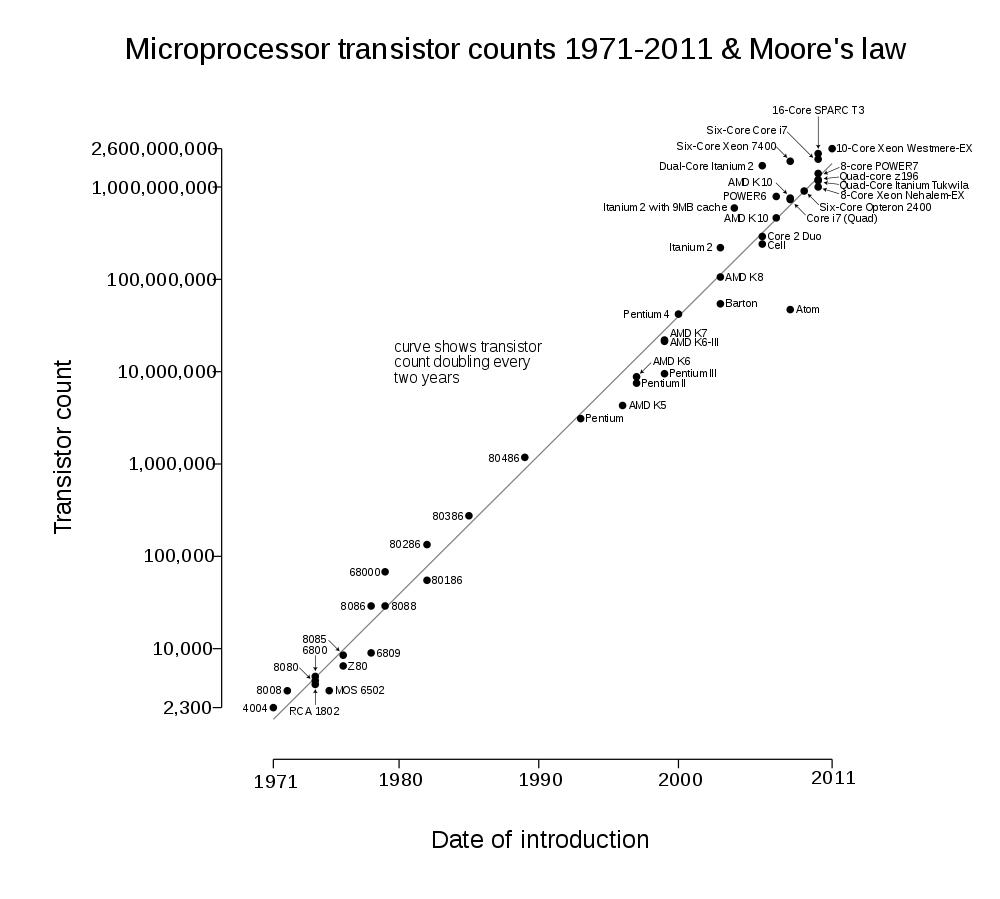
\includegraphics[width=1.1\textwidth]{pictures/figuren/moore_law.png}
%     \caption{De wet van Moore \\ {\small \textit{Wgsimon, CC BY-SA licentie}}}
%     \label{fig:moore-law}
% \end{figure}

% De wet van Moore is te zien in figuur \ref{fig:moore-law}. De schaalverdeling is aangepast op het verloop van de ontwikkelingen door de jaren heen. De figuur dient ter illustratie van de beschrijving in Ledin.



\section{Binair rekenen}

Om getallen te representeren gebruiken we een talstelsel. Een talstelsel is een manier om getallen te representeren, zodanig dat we er mee kunnen rekenen. Mensen maken vaak gebruik van het tientallig (ofwel decimale) talstelsel. De eerste computers deden dit ook, maar al snel bleek dat er betere oplossingen waren in de vorm van het binaire talstelsel.

\subsection{Binair talstelsel}

Het binaire (ofwel tweetallig) talstelsel bestaat slechts uit twee tekens: 0 en 1. Met deze twee tekens moeten alle mogelijke getallen weergegeven worden. Het binaire talstelsel is, net zoals het decimale talstelsel, een positietalstelsel \cite{ou-diwi}. In een dergelijk talstelsel is de positie van een teken bepalend voor de waarde ervan. Dit is te zien wanneer we het decimale getal 125 nemen:
\[
    100 + 20 + 5 = 125
\]
De 5 staat helemaal rechts in het getallen en die positie staat voor het aantal keren dat we 1 tellen (in dit geval 5). Het getal daar links van, 2, staat voor het aantal keren dat we een tien tellen. Het getal daar links van staat voor het aantal keren dat we honderd tellen, enzovoort.

Zoals hierboven is te zien, splitsen we onze getallen op in veelvouden van tien. Het getal is daarom ook als volgt op te splitsen:
\[
    1 \cdot 10^2 + 2 \cdot 10^1 + 5 \cdot 10^0 = 125
\]
Wat we hier hebben gedaan, is het op wiskundige wijze schrijven van het getal met een grondtal. Het grondtal van een talstelsel vormt de basis voor dat stelsel. In het decimale talstelsel is het grondtal 10 (omdat er tien verschillende tekens zijn om uit te kiezen). In het binaire talstelsel zijn er slechts twee, waardoor het grondtal 2 wordt. Een binaire representatie van 125 is dan ook als volgt:
\[
    1 \cdot 2^6 + 1 \cdot 2^5 + 1 \cdot 2^4 + 1 \cdot 2^3 + 1 \cdot 2^2 + 0 \cdot 2^1 + 1 \cdot 2^0 = 125
\]
Om deze representatie te noteren, doen we dit hetzelfde als bij het decimale talstelsel. Het aantal malen dat we daar machten van 10 telden, gaven de tekens welke we noteren op de bijbehorende positie. Zo ook bij het binaire talstelsel, nemen we het aantal keren dat we de machten van twee tellen om het getal te kunnen noteren:
\[
    1111101_2
\]
In Ledin wordt een notatiewijze gegeven voor binaire/hexadecimale getallen door er \texttt{0x} of \textit{h} voor te schrijven. Wat je ook nog wel eens ziet is dat  het grondtal behorende bij een bepaald getal in subscript achter het getal wordt genoteerd (zoals te zien aan de $_2$ bij het binaire getal hierboven). Omdat getallen in het tientallig talstelsel erg gangbaar zijn, noteren we bij getallen in dit talstelsel het grondtal niet.

\begin{opdracht}
Schrijf de getallen 14 tot en met 20 in het binaire stelsel.
\end{opdracht}

\begin{opdracht}
Hoeveel verschillende getallen zijn er in het binaire talstelsel te weergeven met maximaal 5 getallen?
\end{opdracht}

\begin{opdracht}
Schrijf $11111_2$ en $101010_2$ als getallen in het tientallig stelsel.
\end{opdracht}

\begin{opdracht}
Schrijf 52, 91 en 351 als binair getal.
\end{opdracht}

% Met binaire getallen valt ook te rekenen. Bij dit vak kijken we alleen naar het optellen van binaire getallen. Hieronder worden twee voorbeelden gegeven, van een decimale en van een binaire optelling.\\
% \begin{minipage}{.4\linewidth}
% {
% \setlength{\mathindent}{0cm}
% \begin{align*}
% 1101001_2\\
% +\ \ \  100100_2\\
% \text{\rule{2cm}{0.5pt}}\\
% 10001101_2
% \end{align*}
% }
% \end{minipage}
% \mbox{}
% \begin{minipage}{.4\linewidth}
% {
% \setlength{\mathindent}{0cm}
% \begin{align*}
% 125\\
% +\ \ \ 376\\
% \text{\rule{1cm}{0.5pt}}\\
% 501
% \end{align*}
% }
% \end{minipage}\\

% De truc zit hem in wat er gebeurt wanneer je 9 + 1 uitvoert. In dat geval wordt het getal 0 maar komt er 1 voor te staan (10). Zo werkt het ook in het binaire stelsel, maar ditmaal als volgt: $1_2 + 1_2 = 10_2$.

Via de volgende link kun je tevens een leuke YouTube-video bekijken van het kanaal Computerphile, waarin professor David Brailsford een leuke uitleg geeft over binair rekenen: {\color{blue} \url{https://www.youtube.com/watch?v=WN8i5cwjkSE}}.

% \begin{opdracht}
% Tel de binaire getallen $10011101_2$ en $110111011_2$ binair bij elkaar op.
% \end{opdracht}

\subsection{Hexadecimaal talstelsel}

\studeeraanwijzing{Bestudeer in Ledin ``Computer Architecture", paragraaf ``Binary and hexadecimal numbers"\ (\href{https://learning.oreilly.com/library/view/modern-computer-architecture/9781803234519/Text/Chapter_1.xhtml#_idParaDest-27}{link}).}

De uitleg in Ledin is volledig en vooral tabel 1.1 is belangrijk. Deze tabel laat zien wat de hexadecimale variant is van een getal van vier bits. Deze tabel kan gemakkelijk worden gebruikt om binaire getallen om te zetten naar hexadecimale getallen en vice-versa.

\begin{opdracht}
Zet $3A6_{16}$ om in een decimaal getal.
\end{opdracht}

\begin{opdracht}
Schrijf 783 als getal in het hexadecimale stelsel.
\end{opdracht}

\begin{opdracht}
Schrijf $7CE_{16}$ als binair getal.
\end{opdracht}

\begin{opdracht}
Schrijf $0011\ 0101\ 1110\ 1011_2$ als hexadecimaal getal.
\end{opdracht}

% \subsection{2's complement}

% Via de volgende link kun je tevens een leuke YouTube-video bekijken van het kanaal Computerphile, waarin professor David Brailsford een leuke uitleg geeft over 2's complement: {\color{blue} \url{https://www.youtube.com/watch?v=lKTsv6iVxV4}}.

% \intextnote{2's Complement} is de wijze waarop we binnen een computer een negatief getal kunnen representeren. De makkelijkste manier om dat voor te stellen, is het te zien als een speciale indeling van binaire getallen. In de video die hierboven toegevoegd is, wordt vertelt over de verschillende vormen van negatieve getallen binnen een binair talstelsel. Deze hebben allemaal te maken met een \intextnote{sign bit}. Dit is altijd de meest linker bit in een binair getal, welke we bekijken als een + of - (+ = 0, - = 1). Dit is te zien in de volgende getallenlijn.

% % Please add the following required packages to your document preamble:
% % \usepackage{graphicx}
% \begin{table}[h]
% \caption{2's Complement indeling}
% \resizebox{\textwidth}{!}{%
% \begin{tabular}{|l|l|l|l|l|l|l|l|l|l|l|l|l|l|l|l|l|}
% \hline
% 0000 & 0001 & 0010 & 0011 & 0100 & 0101 & 0110 & 0111 & 1000 & 1001 & 1010 & 1011 & 1100 & 1101 & 1110 & 1111 & Binair         \\ \hline
% 0    & 1    & 2    & 3    & 4    & 5    & 6    & 7    & 8    & 9    & 10   & 11   & 12   & 13   & 14   & 15   & Normaal        \\ \hline
% 0    & 1    & 2    & 3    & 4    & 5    & 6    & 7    & -8   & -7   & -6   & -5   & -4   & -3   & -2   & -1   & 2's Complement \\ \hline
% \end{tabular}%
% }
% \end{table}

% Het bijzondere aan deze indeling is dat dezelfde wijze van optellen bij binaire getallen nu ook werkt voor de negatieve getallen.

% \begin{opdracht}
% Tel 3 en -2 in 2's complement bij elkaar op.
% \end{opdracht}

% \begin{opdracht}
% Tel 7 en -4 in 2's complement bij elkaar op.
% \end{opdracht}

\newpage
\section{6502 Processor}

\studeeraanwijzing{Bestudeer in \textbf{Ledin} de paragraaf over ``The 6502 microprocessor" tot het einde van het hoofdstuk (\href{https://learning.oreilly.com/library/view/modern-computer-architecture/9781803234519/Text/Chapter\_1.xhtml\#:-:text=The\%206502\%20microprocessor}{link}).}

\begin{center}
    \fbox{\begin{minipage}{\textwidth-30pt}
    \footnotesize \textbf{N.B.} We gaan er in dit hoofdstuk vanuit dat bekend bent met hexadecimale en binaire getallen. Is dit wat weggezakt? Kijk dan bijvoorbeeld deze video van Bas on Tech:  \url{https://www.youtube.com/watch?v=kG8_L59gmVU}
\end{minipage}}
\end{center}
\vspace{\baselineskip}

De 6502 is te programmeren in een programmeertaal die we assembly language noemen. Deze programmeertaal staat dicht op de hardware en wordt vertaald naar een andere taal welke de processor kan begrijpen. Omdat een processor alleen kan werken met binaire getallen, bestaat die taal dan ook uit enen en nullen. Een dergelijke taal heet machinecode. Machinecode en assembly language zijn beide voorbeelden van \emph{lagere} programmeertalen. Een lagere programmeertaal wordt zo genoemd omdat deze dichter bij de hardware staat. Daarmee bedoelen we dat de taal afhankelijk is van de hardware waar deze voor is gemaakt. Een \emph{hogere} programmeertaal is niet afhankelijk van de processor waar programma's geschreven in deze taal op worden uitgevoerd. Een dergelijke taal is \emph{abstracter} en wordt middels een compiler vaak omgezet naar assembly language om vervolgens te worden omgezet naar machinecode. Deze taak wordt uitgevoerd door een assembler.

De tekst uit Ledin kan hier en daar soms wat lastig zijn. Het is niet belangrijk om na het lezen van de tekst in een keer precies te begrijpen hoe de 6502 processor precies werkt, omdat dit erg lastig is gezien de vele opties die de processor heeft (en dit is nog maar een kleine processor vergeleken met die van vandaag de dag!).

\begin{figure}[!h]
    \centering
    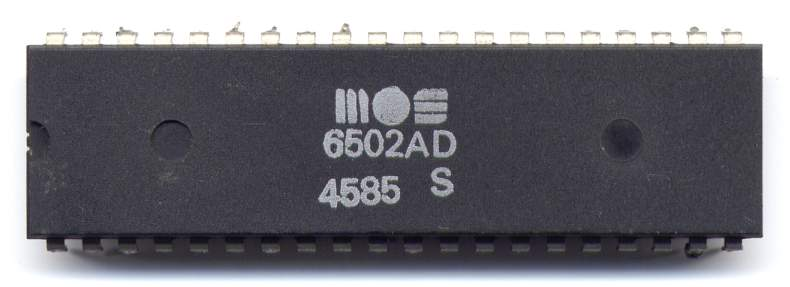
\includegraphics[width=0.5\textwidth]{pictures/figuren/MOS_6502.jpg}
    \caption{MOS 6502 \\ {\small \textit{Dirk Oppelt, CC BY-SA licentie}}}
    \label{fig:MOS6502}
\end{figure}

In Ledin wordt gelinkt naar {\color{blue}\url{https://skilldrick.github.io/easy6502/}}, een online simulator van de 6502. We gebruiken deze pagina ook bij dit vak, omdat dit een goed praktisch begin is om te leren werken met de 6502 processor. Let wel op, omdat dit een erg andere vorm is van programmeren dan je gewend bent vanuit de eerdere vakken die je hebt gevolgd. Feitelijk staan dezelfde mogelijkheden tot je beschikking zoals je die ook kent vanuit de programmeervakken, maar ze werken op een andere, meer gedetailleerde wijze.

Als voorbeeld geven we hieronder een stukje 6502 code die een loop voorstelt. Deze loop wordt gebruikt om kleuren naar het schermpje te schrijven van de 6502 emulator.
\newpage

\begin{lstlisting}[language=asm6502, escapechar=\%]
    LDX #$ff	   ;load $ff in X
    LDA #$01	   ;load $01 in A
loop:              ;loop label
    DEX            ;decrement X
    STA $0200,X	   ;store value in reg A at $0200+X
    ADC #$01	   ;add $01 to A
    TAY            ;copy value of A to Y
    CPY #$0f	   ;compare Y with $0f
    BNE aftercol   ;if not equal, jump to aftercol
    LDA #$00	   ;load $00 in A
aftercol:          ;aftercol label
    CPX #$0        ;compare X with $0
    BNE loop	   ;if not equal, jump to loop
    BRK            ;break
\end{lstlisting}

Om de verschillende instructies te kunnen gebruiken, is een referentie nodig waarin je ze allemaal kunt opzoeken (het zijn er teveel om te onthouden en dat wordt dus ook niet van je verwacht op bijv. de toets). Je kunt de referentie vinden op \href{https://jaar1.schoolofict.nl/}{Blackboard} onder het mapje van dit vak.

\section{Huiswerk}
Maak alle opdrachten tot aan 'Addressing Modes' die worden gegeven op {\color{blue}\url{https://skilldrick.github.io/easy6502/}}.

De opdracht behorende bij het stuk over Adressing Modes en het spelletje aan het eind zijn optioneel en ook geen toetsstof.
